% CREATED BY DAVID FRISK, 2016

% IMPORT SETTINGS
\documentclass[12pt,a4paper]{report}
% CREATED BY DAVID FRISK, 2016
% MODIFIED BY ALEXANDER HÅKANSSON, 2017

% "Variables"
\newcommand{\varthetitle}{Recommending social platform content using deep learning}
\newcommand{\varthesubtitle}{A reccurrent neural network model as an alternative to existing recommender systems}

\usepackage{subcaption}
\usepackage{adjustbox}
\usepackage{multicol}
\usepackage{tabu}
% BASIC SETTINGS
\usepackage{glossaries}                             % Glossarie
\usepackage{moreverb}								% List settings
\usepackage{textcomp}								% Fonts, symbols etc.
\usepackage{lmodern}								% Latin modern font
\usepackage{helvet}									% Enables font switching
\usepackage[T1]{fontenc}							% Output settings
\usepackage[english]{babel}							% Language settings
\usepackage[utf8]{inputenc}							% Input settings
\usepackage{amsmath}								% Mathematical expressions (American mathematical society)
\usepackage{amssymb}								% Mathematical symbols (American mathematical society)
\usepackage{graphicx}								% Figures
\usepackage{subfig}									% Enables subfigures
\numberwithin{equation}{chapter}					% Numbering order for equations
\numberwithin{figure}{chapter}						% Numbering order for figures
\numberwithin{table}{chapter}						% Numbering order for tables
\usepackage{listings}								% Enables source code listings
\usepackage{chemfig}								% Chemical structures
\usepackage[top=2.54cm, bottom=2.54cm,
			inner=3.18cm, outer=2.54cm]{geometry}			% Page margin lengths			
\usepackage{eso-pic}								% Create cover page background
\newcommand{\backgroundpic}[3]{
	\put(#1,#2){
	\parbox[b][\paperheight]{\paperwidth}{
	\centering
	\includegraphics[width=\paperwidth,height=\paperheight,keepaspectratio]{#3}}}}
\usepackage{float} 									% Enables object position enforcement using [H]
\usepackage{parskip}								% Enables vertical spaces correctly 
\usepackage{hyperref}
\hypersetup{
    colorlinks=true,
    linkcolor=blue,
    filecolor=magenta,      
    urlcolor=cyan,
}

\usepackage[
backend=biber,
style=apa,
sorting=nyt,
citestyle=apa 
]{biblatex}
\DeclareLanguageMapping{english}{english-apa}
\DefineBibliographyStrings{english}{%
  references = {References},
}
\addbibresource{references.bib}
 

% OPTIONAL SETTINGS (DELETE OR COMMENT TO SUPRESS)

% Set all fonts to Sans Serif
\renewcommand{\familydefault}{\sfdefault} \normalfont

% Use bold vector notation
\renewcommand{\vec}[1]{\mathbf{#1}}

% Disable hyphenation of text
\tolerance=1
\emergencystretch=\maxdimen
\hyphenpenalty=10000
\hbadness=10000

% Disable automatic indentation (equal to using \noindent)
\setlength{\parindent}{0cm}                         


% Caption settings (aligned left with bold name)
\usepackage[labelfont=bf, textfont=normal,
			justification=justified,
			singlelinecheck=false]{caption} 		

		  	
% Activate clickable links in table of contents  	
\usepackage{hyperref}								
\hypersetup{colorlinks, citecolor=black,
   		 	filecolor=black, linkcolor=black,
    		urlcolor=black}


% Define the number of section levels to be included in the t.o.c. and numbered	(3 is default)	
\setcounter{tocdepth}{5}							
\setcounter{secnumdepth}{5}	


% Chapter title settings
\usepackage{titlesec}		
\titleformat{\chapter}[display]
  {\Huge\bfseries\filcenter}
  {{\fontsize{50pt}{1em}\vspace{-4.2ex}\selectfont \textnormal{\thechapter}}}{1ex}{}[]


% Header and footer settings (Select TWOSIDE or ONESIDE layout below)
\usepackage{fancyhdr}								
\pagestyle{fancy}  
\renewcommand{\chaptermark}[1]{\markboth{\thechapter.\space#1}{}} 


% Select one-sided (1) or two-sided (2) page numbering
\def\layout{1}	% Choose 1 for one-sided or 2 for two-sided layout
% Conditional expression based on the layout choice
\ifnum\layout=2	% Two-sided
    \fancyhf{}			 						
	\fancyhead[LE,RO]{\nouppercase{ \leftmark}}
	\fancyfoot[LE,RO]{\thepage}
	\fancypagestyle{plain}{			% Redefine the plain page style
	\fancyhf{}
	\renewcommand{\headrulewidth}{0pt} 		
	\fancyfoot[LE,RO]{\thepage}}	
\else			% One-sided  	
  	\fancyhf{}					
	\fancyhead[C]{Chapter\nouppercase{ \leftmark}}
	\fancyfoot[C]{\thepage}
\fi


% Enable To-do notes
\usepackage[textsize=tiny]{todonotes}   % Include the option "disable" to hide all notes
\setlength{\marginparwidth}{2.5cm} 


% Supress warning from Texmaker about headheight
\setlength{\headheight}{15pt}		






\begin{document}
% COVER PAGE, TITLE PAGE AND IMPRINT PAGE
\pagenumbering{roman}			% Roman numbering (starting with i (one)) until first main chapter
% CREATED BY DAVID FRISK, 2016
% MODIFIED BY ALEXANDER HÅKANSSON, 2017

% COVER PAGE
\begin{titlepage}
\newgeometry{top=3cm, bottom=3cm,
			left=2.25 cm, right=2.25cm}	% Temporarily change margins		
			
% Cover page background 
\AddToShipoutPicture*{\backgroundpic{-4}{56.7}{figure/front/frontpage-en-GU.pdf}}
\addtolength{\voffset}{2cm}

% Cover picture (replace with your own or delete)		
\begin{figure}[H]
\centering
\vspace{1cm}	% Adjust vertical spacing here
%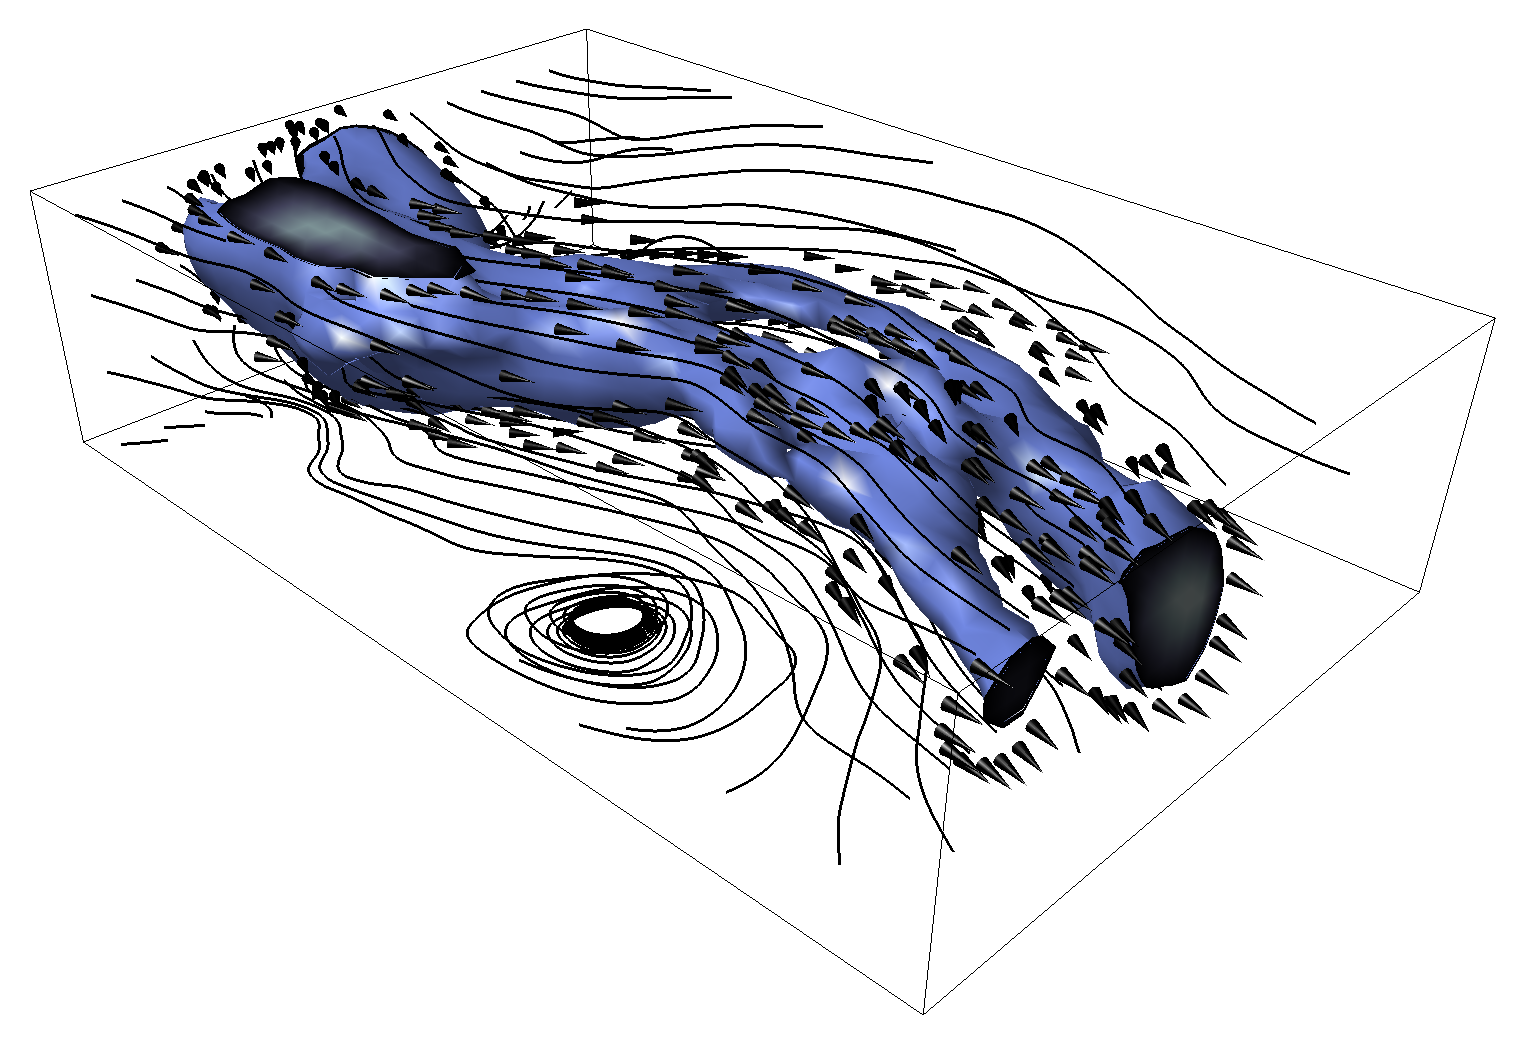
\includegraphics[width=0.9\linewidth]{figure/Wind.png}
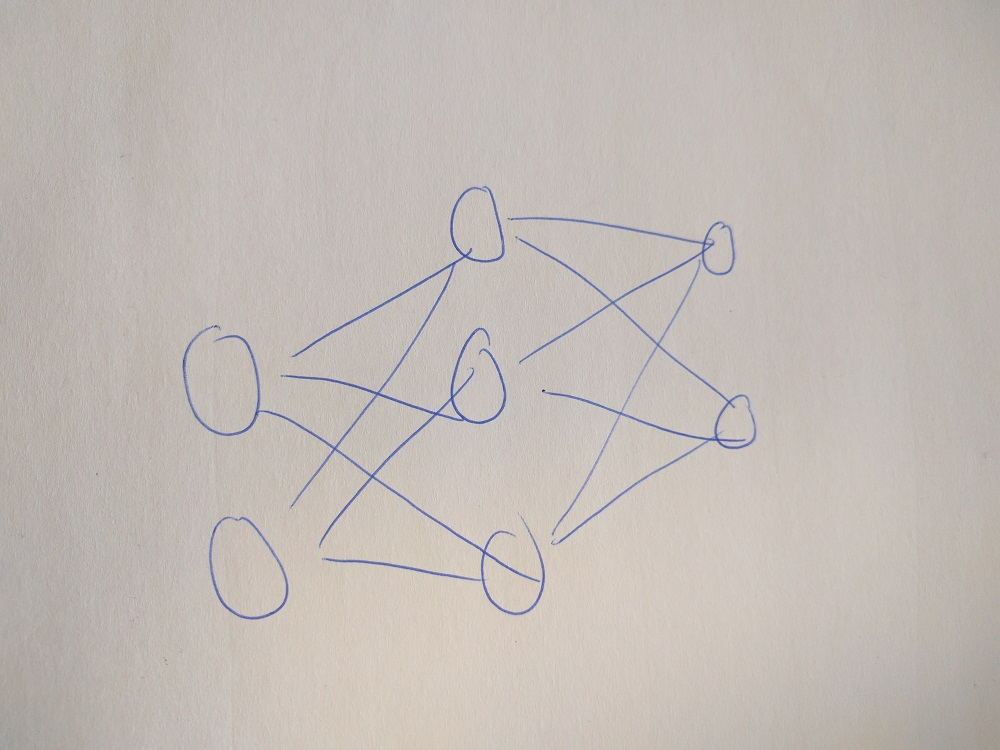
\includegraphics[width=0.9\linewidth]{figure/ann/ann}
\end{figure}

% Cover text
\mbox{}
%\vfill
\renewcommand{\familydefault}{\sfdefault} \normalfont % Set cover page font
\begin{flushleft}
\textbf{{\Huge \varthetitle}} 	\\[0.5cm]
{\LARGE \varthesubtitle}\\[0.2cm]
Bachelor of Science Thesis in Computer Science and Engineering \setlength{\parskip}{0.5cm}

{ JESPER JAXING, ALEXANDER HÅKANSSON, MAXIM GORETSKYY, GMAL TCHAEFA, AXEL OLIVECRONA, JONATAN ALMÉN} \setlength{\parskip}{1.9cm}\\
\vfill
Chalmers University of Technology \\
University of Gothenburg \\
Department of Computer Science and Engineering \\
Göteborg, Sweden, June 2017

\end{flushleft}
%\renewcommand{\familydefault}{\rmdefault} \normalfont % Reset standard font
\end{titlepage}

%\begin{comment} % Remove comment to get blank page
% BACK OF COVER PAGE (BLANK PAGE)
\newpage
\restoregeometry
\thispagestyle{empty}
\mbox{}
%\end{comment}

% TITLE PAGE
\newpage
\setcounter{page}{1}
\thispagestyle{empty}
\begin{center}
	\large Bachelor of Science Thesis\\[4cm]		% Report number given by department 
	\textbf{\large \varthetitle} \\[0.7cm]
	{\large \varthesubtitle}\\[1cm]
	{\large JESPER JAXING}\\
	{\large ALEXANDER HÅKANSSON} \\
	{\large MAXIM GORETSKYY} \\
	{\large GMAL TCHAEFA } \\
	{\large AXEL OLIVECRONA} \\
	{\large JONATAN ALMÉN} \
	
	\vfill	
	% Logotype on titlepage	
	\begin{figure}[H]
	\centering
	% Remove the following line to remove the titlepage logotype
	%
\includegraphics[width=0.2\pdfpagewidth]{figure/front/logo_eng.pdf} \\	
	\end{figure}	\vspace{5mm}	
	
	Department of Computer Science and Engineering \\
	CHALMERS UNIVERSITY OF TECHNOLOGY \\
	University of Gothenburg \\[0.5cm]
	Göteborg, Sweden 2017 \\
\end{center}


% IMPRINT PAGE (BACK OF TITLE PAGE)
\newpage
\thispagestyle{plain}
%\vspace*{4.5cm}
\textbf{\varthetitle}\\
\varthesubtitle
\vspace*{0.5cm}\\
JESPER JAXING\\
ALEXANDER HÅKANSSON\\
MAXIM GORETSKYY\\
GMAL TCHAEFA\\
AXEL OLIVECRONA\\
JONATAN ALMÉN\setlength{\parskip}{0.7cm}

\copyright ~ JESPER JAXING, 2017\\
\copyright ~ ALEXANDER HÅKANSSON, 2017\\
\copyright ~ MAXIM GORETSKYY, 2017\\
\copyright ~ GMAL TCHAEFA, 2017\\
\copyright ~ AXEL OLIVECRONA, 2017\\
\copyright ~ JONATAN ALMÉN, 2017 \setlength{\parskip}{0.5cm}

\todo{Dubbelkolla så detta stämmer}
Examiner: Richard Johansson, Department of Computer Science and Engineering \setlength{\parskip}{1cm}

Department of Computer Science and Engineering\\
Chalmers University of Technology\\
University of Gotehnburg\\
SE-412 96 Göteborg\\
Sweden\\
Telephone: +46 (0)31 772 1000 \setlength{\parskip}{0.5cm}

\vfill
The Authors grants to Chalmers University of Technology and University of Gothenburg the non-exclusive right to publish the Work electronically and in a non-commercial purpose make it accessible on the Internet.\\\\
The Author warrants that he/she is the author to the Work, and warrants that the Work does not contain text, pictures or other material that violates copyright law.\\\\
The Author shall, when transferring the rights of the Work to a third party (for example a publisher or a company), acknowledge the third party about this agreement. If the Author has signed a copyright agreement with a third party regarding the Work, the Author warrants hereby that he/she has obtained any necessary permission from this third party to let Chalmers University of Technology and University of Gothenburg  store the Work electronically and make it accessible on the Internet.


\vfill
% Caption for cover page figure if used, possibly with reference to further information in the report
Cover:\\
A graph visualisation of a simple artificial neural network. See Chapter \ref{chap:ann} for more details. \setlength{\parskip}{0.5cm}

Department of Computer Science and Engineering\\
Göteborg, Sweden 2017


 

% ABSTRACT
\newpage
% CREATED BY DAVID FRISK, 2016
% MODIFIED BY ALEXANDER HÅKANSSON, 2017
\large
\textbf{\varthetitle}\\
\varthesubtitle\\[0.7cm]
JESPER JAXING\\
ALEXANDER HÅKANSSON\\
MAXIM GORETSKYY\\
GMAL TCHAEFA\\
AXEL OLIVECRONA\\
JONATAN ALMÉN\\
\normalsize
\textit{Department of Computer Science and Engineering\\
Chalmers University of Technology\\
University of Gothenburg}\\[0.7cm]
Bachelor of Science Thesis
\setlength{\parskip}{0.5cm}

\thispagestyle{plain}			% Supress header 
\setlength{\parskip}{0pt plus 1.0pt}
\section*{Abstract}
Lorem ipsum dolor sit amet, consectetur adipisicing elit, sed do eiusmod tempor incididunt ut labore et dolore magna aliqua. Ut enim ad minim veniam, quis nostrud exercitation ullamco laboris nisi ut aliquip ex ea commodo consequat. Duis aute irure dolor in reprehenderit in voluptate velit esse cillum dolore eu fugiat nulla pariatur. Excepteur sint occaecat cupidatat non proident, sunt in culpa qui officia deserunt mollit anim id est laborum.

% KEYWORDS (MAXIMUM 10 WORDS)
\vfill
\textbf{Keywords:} lorem, ipsum, dolor, sit, amet, consectetur, adipisicing, elit, sed, do.

\newpage				% Create empty back of side
\thispagestyle{empty}
\mbox{}

% ACKNOWLEDGEMENTS
\newpage
% CREATED BY DAVID FRISK, 2016
\thispagestyle{plain}			% Supress header
\section*{Acknowledgements}
We would like to thank our supervisor Olof Mogren for the great insight and feedback that he has provided during the work with project, making it a fun process and enabling us to succeed. We would also like to thank the division for language and communication for their tremendous help with producing the writing of this thesis. Furthermore, the feedback we have received from other bachelors thesis groups have been of great help.

\newpage				% Create empty back of side
\thispagestyle{empty}
\mbox{}


% TABLE OF CONTENTS
\newpage
\tableofcontents

% OTHER FRONTMATTER
% List of figures (add to table of contents)
\cleardoublepage
\addcontentsline{toc}{chapter}{\listfigurename} 
\listoffigures
% List of tables (add to table of contents)
\cleardoublepage
\addcontentsline{toc}{chapter}{\listtablename}  
\listoftables


% START OF MAIN DOCUMENT
\cleardoublepage
\setcounter{page}{1}
\pagenumbering{arabic}			% Arabic numbering starting from 1 (one)
\setlength{\parskip}{0pt plus 1pt}

\clearpage



% INTRODUCTION
% CREATED BY DAVID FRISK, 2016
\chapter{Introduction}
This chapter presents the section levels that can be used in the template. 

\section{Section levels}
The following table presents an overview of the section levels that are used in this document. The number of levels that are numbered and included in the table of contents is set in the settings file \texttt{Settings.tex}. The levels are shown in Section \ref{Section_ref}.

\begin{table}[H]
\centering
\begin{tabular}{ll} \hline\hline
Name & Command\\ \hline
Chapter & \textbackslash\texttt{chapter\{\emph{Chapter name}\}}\\
Section & \textbackslash\texttt{section\{\emph{Section name}\}}\\
Subsection & \textbackslash\texttt{subsection\{\emph{Subsection name}\}}\\
Subsubsection & \textbackslash\texttt{subsubsection\{\emph{Subsubsection name}\}}\\
Paragraph & \textbackslash\texttt{paragraph\{\emph{Paragraph name}\}}\\
Subparagraph & \textbackslash\texttt{paragraph\{\emph{Subparagraph name}\}}\\ \hline\hline
\end{tabular}
\end{table}

\section{Section} \label{Section_ref}
\subsection{Subsection}
\subsubsection{Subsubsection}
\paragraph{Paragraph}
\subparagraph{Subparagraph}


%Diskutera datan:(notera det här är bara bajs så vi kan diskutera något senare, därför skriver jag på svenska //maxim)
%Vi kunde få ut X antal interaktioner med trådar på reddit, där en interaktion motsvarar en downvote eller upvote.Varje interaktion är kopplad till en specific person i datasettet. Vi får också ut vilken subreddit tråden var skapad på, och eventuell innehåll(content).
\\ %Den här kan typ vara i terminologi, eftersom vi endast förklarar hur datan ser ut.
%I första modellen tog vi bara ut de "positiva" interaktioner, dvs alla med upvotes, och grupperade datan så att varje titel har ett set av användarna (i postgres). För att träna den första modellen var vi bara intresserade av titeln och användarna, dvs titel var vår inputdata och mängden av användarna var vår "target"/"labeled" data, dvs den outputten som vi vill att den ska få. 
%tl;dr input = titel, output = användarna som är intresserade.
\\
%En annan ide är att även använda de negativa interaktioner(downvotes), man kan tolka det på olika sätt: en downvote kan vara att du är inte intresserad av det och då borde man straffa modellen mer om en användare ger en downvote på en titel, det andra sättet och tolka är på är att man är intresserad men håller inte med personen eller tycker inte om sättet någon beskrev det på, men själva ämnet är fortfarande intressant. Det leder till två olika modeller/approaches som man kan undersöka.
\chapter{Theory}
\section{Optimisation}
\subsection{Gradient descent, tractability}%Tractability?
Gradient descent is an optimisation method where one calculates the gradient of a function and then takes a small step in the opposite direction of the gradient, this is repeated until one has found a local (or global) minimum i.e. the gradient is 0. It has been shown that this works well for convex(?) functions[source] since convex functions have the property that every local minimum is also a global minimum . However, an artificial neural network is not a convex function, but much more complicated.[source] Therefore gradient descent should not be a good method to use in this case, but empirical proof shows that it work well. %Vi ska inte ge vår åsikt här, räcker att säga att Det finns emperiska bevis som säger att gradient descent är bra och ha källa.
When talking about artificial neural networks it is the gradient of the error function that is interesting. Calculating the gradient of the error function with regards to the weights of the network will give an indication as to whether to decrease or increase the weights. This is how the network learns what is good and what is bad, by changing its weights to minimise the error function.
\subsection{Backpropagation}
Backpropagation is a method used when training ANNs. When a you feed a vector into the network it will propagate forward until in reaches the last layer and presents an output. The output is then compared to the desired result via an error function to determine how well the network performed on the given output. It is now that backpropagation will start. Each neural will be assigned an error, the error will then propagate backwards through the network and the weights will be updated. How the weights are updated depends on what optimisation method is used.
\section{Classification}
The most common use for machine learning is classification. It is the problem of given a new data point classify it as one of the k sets that the machine learning algorithm knows. This problem can be solved with most machine learning models. It can be a quite simple problem and often do not require the use of an ANN. %Är det ett verkligen ett "simple problem", beror ju på vad du vill klassificera
\section{Artificial Neural Networks (ANN)}
An Artificial neural network is an attempt to image the workings of a human brain. The network is constructed of nodes which are structured in layers. The nodes take some input and does something with it and feeds it to the next layer, until it gets to the final layer and outputs something interesting. Between the nodes there are weights, this is what the ANN learns. By using gradient descent and back propagation to change the weights to minimise the error the network will give the right answer more often. 

\subsection{Activation function}
The activation function controls how much of the output from a node is ON. For example if using signum(x) as our activation function then all positive outputs are ON and all negative are off. In order to achieve better results one has to allow more sophisticated outputs than simple ON/OFF-modes. By using non-linear functions you can squash/scale the output. One of the requirements for the network to learn well is to have an activation function that is differentiable in many points.
\subsubsection{Sigmoid} %Vi kan max ha 3 nivåer, så vi får itemizea denna
Sigmoid function is a non-linear function defined by $f(x)=\frac{1}{1+exp(-x)}$ that scales the output between [-1, 1]. 
\subsubsection{ReLU}
ReLU function is a non-linear function defined by $f(x) = max(0,x)$. This function has the benefit of being unbounded as opposed to sigmoid for example whose domain is the interval $[-1, 1]$.  
\subsubsection{Softmax}
Softmax function is defined by $f(x_j) = \frac{e^{x_j}}{\sum_{i=1}^{n} e^{x_i}} $ where $\mathbf{x}$ is a vector of $n$ outputs. Softmax scales the vector entries to be between 0 and 1, while making them sum to 1 because of the normalisation.

\section{Recurrent Neural Network (RNN)}
A recurrent neural network is network that takes time into account. It accounts for time in the sense that the current output is dependent on the previous. This time dependency is often depicted as an ANN that outputs to itself, in reality this is not very useful since it makes the methods for learning (backpropagation) useless. Instead of using a recursive unit, recurrent nets are often modelled as one unit outputing to the next unit in the layer, this unit takes some new input and the output from the previous unit. This processes is called unfolding.%recursive unit? Wut?
\subsection{LSTMs}
\section{Error functions} %Tycker det borde ligga under ANN delen?
\subsection{Mean Squared Error}
The mean squared error function is defined by: $E=\frac{1}{2n}\sum_{i=1}^{n} (target_i - output_i)^2$ where $n$ is amount of inputs that you give to the error function. 
\subsection{Cross Entropy}
Cross entropy function is defined by XXXXX. 

\subsection{Downvote and Upvotes} %Borde inte finnas här, tillhör inte teorin. En del av metod eller diskussion.
The network is currently learning to predict which reddit users are interested in a given title of a reddit post. It learns this by looking at the interactions that users have had with similar posts. If user have upvoted a post that clearly means that the user found the post enjoyable or interesting, but what if the user has downvoted the post or not interacted at all with it? If a user have downvoted a post that could mean one of two things; either the user did not like the content and do not what to see similar posts again or the user find the post interesting but does not agree with the point of view of the poster, in this case the user most likely want to see more similar posts. Similarly with no interaction, a user might simply not have seen the post not liked it or not cared enough to upvote it. This is a problem of social studies, how do user use their downvote?
\section{Training}
Kanske något om hur man kan utnyttja downvotes
\chapter{Method}%Är metod och utförande samma sak?
This chapter will describe the workprocess of this project and what has been done.
\section{Deciding on a dataset}
måste vara naturligt labeled
\subsection{Ubuntu dialogue corpus}
This data set consists of back and forth conversations between users. Even thought the dataset is large it is not natural labeled for our needs and it is not clear how training on back and forth conversations would help it prediction what users would find a post on the web interesting. The Ubuntu dialogue corpus was ultimately not used since the data was not suited to our task.
\subsection{Reddit}
\section{Gathering data}
något om att deep ann:s behöver mycket data %Must be mentioned in theory part
\section{Modeling as an RNN}
\subsection{Tensorflow}%The explanation about tensorflow should be made in terminology, here we shall only name how we will use it.
Tensorflow is a high level framework, developed by Google to give the possibility of developing machine learning applications without having a deep knowledge. %även om det är sant att man inte behöver vara ML proffs tycker jag det får oss att låta dumma% 
\subsection{LSTM-network}
\subsection{Scaling down}
As by suggestion from our supervisor we will begin with a very small scale network, instead of having the number of users in the tens of thousands we will start with 2-5 users. The reasoning for this is it that it will now be easier to not just train the network but to also to analyse it. This is a common approach in machine learning (source Olof) and the hope is that whatever model works on the small scale will hopefully continue to perform when it is scaled up.    
\subsection{Overfitting on purpose}
Overfitting is something you want to avoid in the final model but can be useful in development. Overfitting is a result of having learnt the training data too well but the key here is that something has been learnt. If the model has learnt something you at least know you are on the right path, it is not making guesses at random. Overfitting is therefore the first milestone for our scaled down network. 
\subsection{Scaling up}
\subsection{Tuning hyperparameters}
\section{Baseline}
When deciding how well a model performs it is compared against a baseline. The baseline puts the accuracy of the model into some context. You might have an accuracy of 90\%, is that good or bad? You need one or more baselines to decide this. 
\subsection{Random classifier}
A random classifier is a model that given an input $x$ selects one of $n$ output values uniformly at random. This results in an expected accuracy of $\frac{1}{n}$. This is a baseline that any real life model needs to beat with confidence.
\subsection{Collaborative filtering}
%Flytta förklaringen till ordlista? 
Collaborative filtering can be used in what is called recommender systems. The goal of a recommender system is to recommend users products that the user finds interesting or helpful. Collaborative filtering operates under the assumption that if Bob likes cats and dogs and Alice likes cats, Alice is more likely to also like dogs since Bob likes dogs and Alice share a interest with Bob. Collabortive filtering has found success in recommending items such as movies (netflix prize source). %Kanske något mer om hur vi använde detta som baseline%

\subsection{N-gram}
\section{Computing power restrictions} %Should 
\section{Integration with an application}


%Saker som man är också intressanta: Kolla upp variansen, debugg, hur vi hitta felet etc. 
\chapter{Results}\label{chap:results}
This chapter will present the results achieved in the project as described in Chapter \ref{chap:method}. These results includes comparisons between different models and their hyperparameters but also a look at the different datasets that were used.

\section{Analysis of the datasets}
\label{sec:dataset-summary}
The purpose of this section is to present the result of an investigation into the different datasets. The goal of this was to see if there were any irregularities or patterns in the datasets that could have had an affect on the performance of the networks or the baselines. 
\subsection{5 user data set allvotes}
\label{sec:five-user-data-set}

One thing that we found in the training set for the five user dataset was that the difference in length of the longest title and the second longest title was large. The longest title was 1928 words while the second longest was 66 words. This skewed the variance for the training data and is why one standard deviation sits at $24.9$ as you can see in \ref{table:5-user-set-train} while all the other datasets sits around $10$. If the outlier is removed, one standard deviation is brought down to $9.7$ and sits around the same value as all the other.
\\\\
Another point of interest is how few users share liked titles. In the training set \ref{table:5-user-set-train} you can see that only about $1\%$ of titles have more than 1 up or downvote. In the validation \ref{table:5-user-set-train} and test set \ref{table:5-user-set-train} it is even less titles, $0.45\%$ for the validation and $0.6\%$ for the test set.
\\\\
The data regarding the vote density in subreddits for the $50$ users datasets have been left out simply due to the size of the tables they would require, the data is however available in appendix \ref{appendix:dataset} if the reader is interested.


\begin{table}[H]
    \centering
    \begin{tabular}{ r | c | c | p{4cm}  }
    \hline
    \textbf{User} & \textbf{Active subreddits} & \textbf{Total votes} & \textbf{Votes in two most voted subreddits} \\ \hline \hline
    \multicolumn{4}{c}{\textbf{Training data set}} \\ \hline \hline
    Ayavaron & 64 & 1411 & 444 \\ \hline
    akkartik & 14  & 1387 & 1333 \\ \hline
    crmaki & 14 & 1410 & 902 \\ \hline
    izzycat & 37 & 1363 & 505 \\ \hline
    doctorgonzo & 32 & 1429 & 586 \\ \hline \hline
    \multicolumn{4}{c}{\textbf{Validation data set}} \\ \hline \hline
    Ayavaron & 40 & 416 & 133 \\ \hline
    akkartik & 8  & 392 & 372 \\ \hline
    crmaki & 11 & 390 & 252 \\ \hline
    izzycat & 26 & 428 & 158 \\ \hline
    doctorgonzo & 24 & 364 & 146 \\ \hline \hline
    \multicolumn{4}{c}{\textbf{Testing data set}} \\ \hline \hline
    Ayavaron & 33 & 172 & 60 \\ \hline
    akkartik & 5  & 220 & 212 \\ \hline
    crmaki & 12 & 194 & 131 \\ \hline
    izzycat & 19 & 207 & 77 \\ \hline
    doctorgonzo & 28 & 204 & 78 \\ \hline
    \end{tabular}
    \caption{Vote distribution for the training, validation and testing data sets with five users}
    \label{table:5_user_reddit_dataset}
\end{table}
\todo{Dubbel kolla siffrorna}
\begin{table}[H]
    \centering
    \begin{tabular}{ r | c | c | c }
    \hline
    \textbf{Feature} & \textbf{Training} & \textbf{Validation} & \textbf{Testing} \\ \hline \hline
    \multicolumn{4}{c}{\textbf{Titles}} \\ \hline \hline
    Amount & 6927 & 1983 & 992 \\ \hline
    Median length & 9 & 9 & 8 \\ \hline
    Average length & 12 & 11 & 11  \\ \hline
    Within $\sigma$ title length & 24.9 & 9.6 & 9.4 \\ \hline
    Longer than average & 2198 & 696 & 320 \\ \hline
    More than 1 vote & 76 & 9 & 6 \\ \hline
    More than 2 votes & 2 & 0 & 0\\ \hline \hline
    \multicolumn{4}{c}{\textbf{Subreddits}} \\ \hline \hline
    Amount & 103 & 65 & 59  \\ \hline
    Average voted in in & 32.2 & 21.8 & 19.4 \\ \hline
    Within $\sigma$ voted in & 18.4 & 11.49 & 10.2  \\ \hline
    \end{tabular}
    \caption{Statistics for the dataset containing five users}
    \label{table:5-user-set-train}
\end{table}
\subsection{50 user data set allvotes}
Here there are not any big outliers in title length as in the five user dataset but there is a higher percentage of users that share liked titles compared to the five user dataset. In the training set for the fifty user dataset, $7.75\%$ of titles have more than one up or downvote. In the validation set it is $6\%$ and for the testing set it is $5.7\%$.


\begin{table}[H]
    \centering
    \begin{tabular}{ r | c | c | c }
    \hline
    \textbf{Feature} & \textbf{Training} & \textbf{Validation} & \textbf{Testing} \\ \hline \hline
    \multicolumn{4}{c}{\textbf{Titles}} \\ \hline \hline
    Amount & 63176 & 18486 & 9301 \\ \hline
    Median length & 9 & 9 & 9 \\ \hline
    Average length & 12 & 12 & 12  \\ \hline
    Within $\sigma$ title length & 11.7 & 9.3 & 9.3 \\ \hline
    Longer than average & 23474 & 6736 & 3354 \\ \hline
    More than 1 vote & 5428 & 1231 & 577 \\ \hline
    More than 2 votes & 980 & 220 & 92\\ \hline \hline
    \multicolumn{4}{c}{\textbf{Subreddits}} \\ \hline \hline
    Amount & 343 & 248 & 192  \\ \hline
    Average voted in in & 31.28 & 22.6 & 18.58 \\ \hline
    Within $\sigma$ voted in & 17.6 & 12.17 & 9.88  \\ \hline
    \end{tabular}
    \caption{Statistics for the dataset containing fifty users}
    \label{table:50-user-set-train}
\end{table}

\todo{moar plots/graphs}

As seen in figure \ref{fig:histvotes} most of the posts have a low number of upvotes, this could potentially mean that it is hard to learn from this data.

\begin{figure}[H]
    \centering
    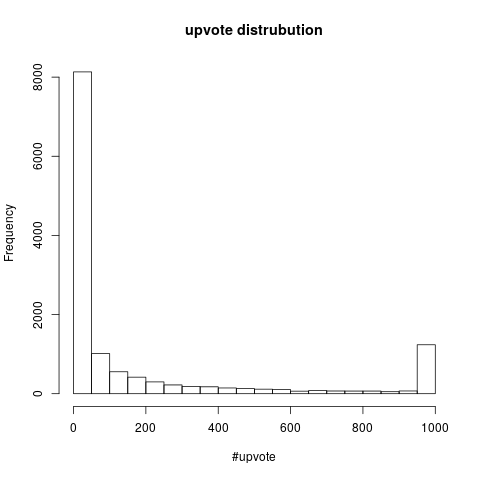
\includegraphics[width=0.75\textwidth]{figure/results/histupvote}
    \caption{A histogram with number of upvote per post on the x axis and number of posts on the y axis.}
    \label{fig:histvotes}
\end{figure}


\section{The first iteration model}
The first iteration of the model was implemented with no hidden layers, as described in section \ref{sec:modelling_the_ann}. It had an LSTM-RNN layer as its input layer with 30 LSTM units. Full details on this model are found in section \ref{sec:app2_first_iter}. When this model was trained on a dataset downscaled to contain five users overfitting was achieved as shown in figure \ref{fig:first_iter_overfitting}.
\begin{figure}[h!]
\begin{subfigure}{0.5\textwidth}
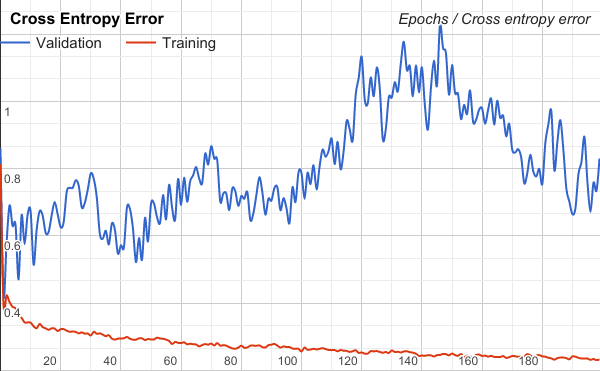
\includegraphics[width=1 \linewidth]{figure/results/first_iter_cross}
\caption{Cross entropy error}
\label{fig:first_iter_overfitting}
\end{subfigure}
\begin{subfigure}{0.5\textwidth}
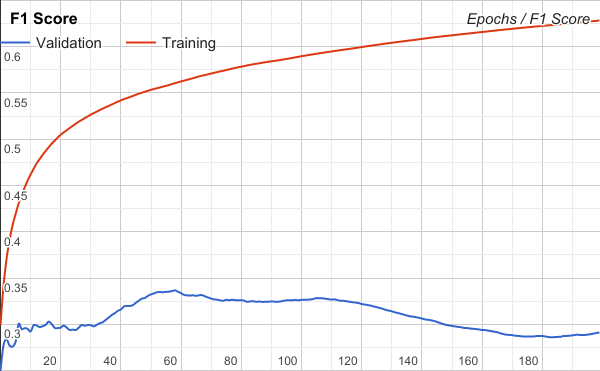
\includegraphics[width=1\linewidth]{figure/results/first_iter_f1}
\caption{$F_1$ score.}
\label{fig:first_iter_f1}
\end{subfigure}
 
\caption{The cross entropy error and $F_1$ score of the first iteration model after 200 training epochs, trained on the training and validation sets. It is good to achieve a low error and a high $F_1$. $F_1$ ranges between $0$ and $1$ inclusive.}
\label{fig:image2}
\end{figure}
\\
The best $F_1$ score achieved on the validation set using the model was $0.3366$, as shown in figure \ref{fig:first_iter_f1}, but the main takeaway was that the model is able to learn from the data.

\section{The final network}
The most optimal network we managed to achieve for the five user dataset had an accuracy of about $39\%$. Even after 1470 epochs this model had not overfitted, however the performance hardly got better after more epochs.

\subsection{Hyperparamaters}
The final result of the hyperparamaters are shown in table \ref{table:hyperparameters_final}

\begin{table}[h!]
    \centering
    \begin{tabular}{ r  p{7cm} }
        \hline
        \textbf{Hyperparamter}  &  \textbf{Value} \\ \hline \hline
        Learning rate & $0.05$  \\ \hline
        Batch Size & $25$ \\ \hline
        RNN units & $400$  \\ \hline
        Embedding Size & t $300$ \\ \hline
        Pre-trained embedding matrix & $False$ \\ \hline
        Trainable embedding matrix & $True$ \\ \hline
        Hidden layers & $1$ \\ \hline
        Neurons in hidden layers & $300$ \\ \hline
        Use L2 regularisation & $True$ \\ \hline
        L2 Factor & $0.01$ \\ \hline
        Dropout regularisation & $True$\\ \hline
        Dropout probability & $0.75$ \\ \hline
        Use constant prediction limit & $False$ \\ \hline
        Constant prediction limit & N/A  \\ \hline
        Use subreddit input & $False$ \\ \hline
    \end{tabular}
    \caption{Final value for all hyperparamaters}
    \label{table:hyperparameters_final}
\end{table}
\section{Baseline comparison} 
\todo{lägga in fina tabeller}
\subsection{Facebook fastText classifier}

\subsection{Random classifier}

\subsection{N-grams}
The F1-score of $0.3898$ was achieved with n-grams when performing on the dataset with five users.
\todo{kör testet med 50 användare sen, GLÖM INTE PLSPLSPLSPLSPLSPLS}


Skriva om hur det gick overall, jämför hur det fungerade med/utan downvotes. vilka hyperparametrar fungerar bar osv.
\chapter{Discussion}


% REFERENCES / BIBLIOGRAPHY
\cleardoublepage
\addcontentsline{toc}{chapter}{Bibliography}
% CREATED BY DAVID FRISK, 2016
\begin{thebibliography}{69}

\bibitem{Reference} Frisk, D. (2016) A Chalmers University of Technology Master's thesis template for \LaTeX . Unpublished.

\end{thebibliography}


% APPENDICES
\cleardoublepage
\appendix
\setcounter{page}{1}
\pagenumbering{Roman}			% Capitalized roman numbering starting from I (one)

\chapter{The Reddit dataset}\label{appendix:reddit}
The Reddit dataset was retrieved from \url{https://www.reddit.com/r/redditdev/comments/bubhl/csv_dump_of_reddit_voting_data/}. The dataset was published by the user \textit{ketralnis} who is an employed administrator on Reddit. The data comes directly from the official Reddit databases.
\\\\
The raw data as retrieved contained three fields per data point which represent a user, a post ID and a vote. Every data point in the dataset indicates that a specified user has either up- or down-voted a certain post on Reddit. An excerpt from the dataset looks like shown in Table \ref{table:reddit_raw_excerpt}.
\begin{table}[h!]
    \centering
    \begin{tabular}{ c c c } 
        \hline
        \textbf{Username} & \textbf{Post ID} & \textbf{Vote} \\
        \hline
        \multicolumn{3}{c}{\vdots} \\
        2bornot2b & t3\_899vr & 1 \\
        2bornot2b & t3\_89as2 & -1 \\
        2bornot2b & t3\_89az7 & 1 \\
        2bornot2b & t3\_89b84 & 1 \\
        2bornot2b & t3\_89c4k & 1 \\
        2bornot2b & t3\_89de8 & -1 \\
        2bornot2b & t3\_89e1e & 1 \\
        \multicolumn{3}{c}{\vdots} \\
    \end{tabular}
    \caption{An excerpt from the raw dataset with the field username, post ID and vote.}
    \label{table:reddit_raw_excerpt}
\end{table}
\\
This raw dataset contains $7,405,561$ votes for a total of $31,927$ users and $ 2,046,401$ posts. The dataset only contains votes from users who have actively agreed to make their votes public. The dataset contains up to the latest $1000$ up- and down-votes (for a maximum of $2000$ votes) for each user. The action to either upvote or downvote a post on Reddit is used on the website to rank posts against eachother where an upvote indicates that a user likes a post and a downvote indicates the opposite. 
\begin{figure}[h]
    \centering
    
\includegraphics[width=0.75\textwidth]{figure/reddit/reddit_voting}
    \caption{An example of a post on Reddit and how it can be either up- or down-voted. Screenshot from \url{http://reddit.com/} on April 4, 2017.}
    \label{fig:example_reddit_post}
\end{figure}
\\\\
The posts on Reddit are written by users on the platform. A post always has a title, and it always belongs to a so called \textit{subreddit}. The post seen in Figure \ref{fig:example_reddit_post} has the title \textit{Colorized by me: Abraham Lincoln, June 3, 1860} and it belongs to the subreddit \textit{pics}. A subreddit can be seen as a category -- there are many subreddits on Reddit and posts belonging to the same subreddit are usually similar.





\end{document}